\documentclass[xcolor=table]{beamer}
\usetheme{Goettingen}

\usepackage[utf8]{inputenc}
\usepackage{graphicx}
\usepackage{color}
\usepackage{booktabs}
\usepackage{tikz}
\usepackage{wrapfig}
\usepackage{caption}
\captionsetup{labelformat=empty}

\title{O Problema do Carteiro Chinês}
\subtitle{Tópicos Especiais em Economia Matemática}
\author{Monitor: Gustavo de Oliveira\\ Orientador: Diogo Bravo Mmarinho Braga}
\institute{Universidade Federal Fluminense - Faculdade de Economia}
\date{}

\begin{document}

\begin{frame}{}
\titlepage
\end{frame}

\begin{frame}{Sumário}
\tableofcontents
\end{frame}

\begin{frame}{Introdução}
\section{Introdução}
\begin{block}{No que consiste o problema? }
O problema do carteiro chinês é um problema de otimização em grafos que consiste em encontrar o caminho de menor custo iniciado em um vértice $i$, passando por \textit{todas} as arestas e retornando ao mesmo vértice, dado que as arestas tem pesos e o grafo é conexo .  \\
\end{block}

As aplicações desse problema estão dentre as mais variadas, podendo estar presentes desde implicações em coletas de lixo as, até mesmo, linhas aéreas.

\end{frame}

\begin{frame}{Identificação do Problema}
\section{Identificação do Problema}
\begin{block}{Como indentificar o problema?}
Dado um grafo conexo G, são duas as coisas Intrínsecas a esse problema que podem acontecer:
    \begin{itemize}
        \item O grafo ser Euleriano ($\delta(v_{i}) = par$) - de tal forma que já haveria uma solução ótima para o problema.
        \item O grafo não ser Euleriano, sendo o caso em que trabalharíamos com o problema do carteiro chinês.
    \end{itemize}
\end{block}
\end{frame}

\begin{frame}{O Algoritmo }
\section{O Algoritmo}
\begin{block}{A Solução}
A solução para o problema do carteiro chinês - com arestas de pesos positivos e não direcionadas - consiste num algoritmo que transforme o grafo não-Euleriano num Grafo Euleriano, por meio de um acréscimo de arestas ``artificiais'', entre os vértices de grau impar do grafo. A partir daí, passa-se a ter uma solução ótima, tal qual para qualquer grafo euleriano. 
\end{block}     
\end{frame}

\begin{frame}{O Algoritmo }
O algoritmo se dá da seguinte forma:

\begin{enumerate}
    \item Determinar os vértices de grau ímpar.
    \item Por meio do algoritmo de \textit{Dijkstra} construir uma matriz de distância D para os vértices de grau ímpar.
    \item Determinar, por meio da matriz D, os vértices $v_{i}$ e $v_{j}$ ímpares de menor caminho.
    \item Acrescentar arestas artificiais de $v_{i}$ para $v_{j}$ com o \textit{custo} obtido pela matriz D. 
    \item Eliminar da matriz D as colunas e linhas correspondentes a $v_{i}$ e $v_{j}$.
    \item Se ainda assim houver vértices ímpares, retornar ao passo 3.
    \item O custo total percorrido será igual ao custo inicial do grafo G somado com o custo das arestas acrescidas.
\end{enumerate}
    
\end{frame}

\begin{frame}{Exemplo}
\section{Exemplo}
Dado o Grafo G abaixo, determinaremos o menor custo possível, 

\begin{wrapfigure}{l}{0\textwidth}
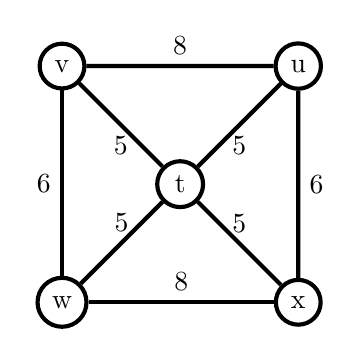
\begin{tikzpicture}[scale = 1.5, line width = 1.5pt]
\draw (0,2) node[circle, draw](a1){v}
    (2,2) node[circle, draw](a2){u}
    (2,0) node[circle, draw](a3){x}
    (0,0) node[circle, draw](a4){w}
    (1,1) node[circle, draw](a5){t};
    \draw [-] (a1) -- (a2) node[midway,above] {8};
    \draw [-] (a1) -- (a4) node[midway,left] {6};
    \draw [-] (a1) -- (a5) node[midway,below] {5};
    \draw [-] (a2) -- (a3) node[midway,right] {6};
    \draw [-] (a2) -- (a5) node[midway,below] {5};
    \draw [-] (a3) -- (a4) node[midway,above] {8};
    \draw [-] (a3) -- (a5) node[midway,above] {5};
    \draw [-] (a4) -- (a5) node[midway,above] {5};
\end{tikzpicture}    
\end{wrapfigure}

\noindent \begin{enumerate}
    \item A primeira coisa a ser feita é determinar os vértides de grau ímpares para, então, criarmos uma matriz D de distância. Os vértices ímpares são: $V_{impar} = \{v, u, w, x\}$
\end{enumerate}
\end{frame}

\begin{frame}{}

Selecionamos os vértices ímpares do grafo G.  

\begin{wrapfigure}{l}{0\textwidth}
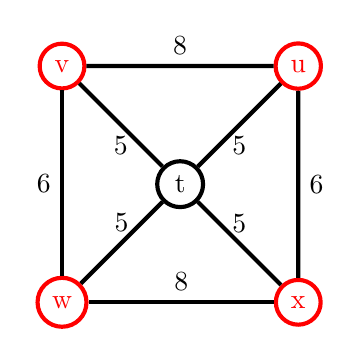
\begin{tikzpicture}[scale = 1.5, line width = 1.5pt]
\draw (0,2) node[circle, draw, red](a1){v}
    (2,2) node[circle, draw, red](a2){u}
    (2,0) node[circle, draw, red](a3){x}
    (0,0) node[circle, draw, red](a4){w}
    (1,1) node[circle, draw](a5){t};
    \draw [-] (a1) -- (a2) node[midway,above] {8};
    \draw [-] (a1) -- (a4) node[midway,left] {6};
    \draw [-] (a1) -- (a5) node[midway,below] {5};
    \draw [-] (a2) -- (a3) node[midway,right] {6};
    \draw [-] (a2) -- (a5) node[midway,below] {5};
    \draw [-] (a3) -- (a4) node[midway,above] {8};
    \draw [-] (a3) -- (a5) node[midway,above] {5};
    \draw [-] (a4) -- (a5) node[midway,above] {5};
\end{tikzpicture}    
\end{wrapfigure}

\noindent \begin{enumerate}[2]
    \item Nosso objetivo agora é construir uma matriz de distância D, para os vértices selecionados, utilizando, para tal, o algoritmo de ``Dijkstra''.
\end{enumerate}
\end{frame}

\begin{frame}{O Algoritmo de Dijkstra}
\section{O Algoritmo de Dijkstra}  
O algoritmo de Dijkstra foi um algoritmo criado por \textbf{Edsger Wybe Dijkstra} e tem como objetivo solucionar o problema de menor custo em relação as arestas entre um vértice $v_{i}$ e $v_{j}$. Utilizemos o algoritmo - de forma prática - para entendermos melhor.

\begin{wrapfigure}{l}{0\textwidth}
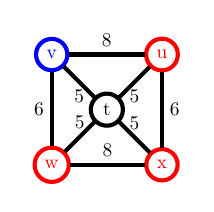
\begin{tikzpicture}[scale = .7, line width = 1.5pt]
\draw (0,2) node[circle,scale = .7, draw, blue](a1){v}
    (2,2) node[circle,scale = .7, draw, red](a2){u}
    (2,0) node[circle,scale = .7, draw, red](a3){x}
    (0,0) node[circle,scale = .7, draw, red](a4){w}
    (1,1) node[circle,scale = .7, draw](a5){t};
    \draw [-] (a1) -- (a2) node[midway,scale = .7,above] {8};
    \draw [-] (a1) -- (a4) node[midway,scale = .7,left] {6};
    \draw [-] (a1) -- (a5) node[midway,scale = .7,below] {5};
    \draw [-] (a2) -- (a3) node[midway,scale = .7,right] {6};
    \draw [-] (a2) -- (a5) node[midway,scale = .7,below] {5};
    \draw [-] (a3) -- (a4) node[midway,scale = .7,above] {8};
    \draw [-] (a3) -- (a5) node[midway,scale = .7,above] {5};
    \draw [-] (a4) -- (a5) node[midway,scale = .7,above] {5};
\end{tikzpicture}    
\end{wrapfigure}

\noindent Dado o vértice $v$, queremos, então, construir uma matriz de distância relativa à esse vértice. Uma observação, se as distâncias possuissem pesos negativos, não utilizaríamos o algorítmo de Dijkstra, teríamos que utilizar o algoritmo de \textbf{Bellman-Ford}. Segue o algoritmo no próximo slide. 

\end{frame}

\begin{frame}{O Algoritmo de Dijkstra}

\begin{center}
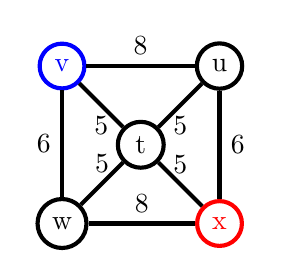
\begin{tikzpicture}[scale = 1, line width = 1.5pt]
\draw (0,2) node[circle,scale = 1, draw, blue](a1){v}
    (2,2) node[circle,scale = 1, draw](a2){u}
    (2,0) node[circle,scale = 1, draw, red](a3){x}
    (0,0) node[circle,scale = 1, draw](a4){w}
    (1,1) node[circle,scale = 1, draw](a5){t};
    \draw [-] (a1) -- (a2) node[midway,scale = 1,above] {8};
    \draw [-] (a1) -- (a4) node[midway,scale = 1,left] {6};
    \draw [-] (a1) -- (a5) node[midway,scale = 1,below] {5};
    \draw [-] (a2) -- (a3) node[midway,scale = 1,right] {6};
    \draw [-] (a2) -- (a5) node[midway,scale = 1,below] {5};
    \draw [-] (a3) -- (a4) node[midway,scale = 1,above] {8};
    \draw [-] (a3) -- (a5) node[midway,scale = 1,above] {5};
    \draw [-] (a4) -- (a5) node[midway,scale = 1,above] {5};
\end{tikzpicture}    
\end{center}

\noindent \begin{table}[]
\centering
\caption{Matriz de Distância de $v-x$}
\label{my-label}
\begin{tabular}{|l|l|l|l|l|l|}
\hline
vértice & peso1                  & peso2 & peso3 & peso4 & peso5 \\ \hline
v       &                        &       &       & &      \\ \hline
u       &                        &       &       &  &     \\ \hline
w       &                        &       &       &   &    \\ \hline
x       &                        &       &       &    &   \\ \hline
t       &                        &       &       &     &  \\ \hline
\end{tabular}
\end{table}
\end{frame}

\begin{frame}{O Algoritmo de Dijkstra}

\begin{center}
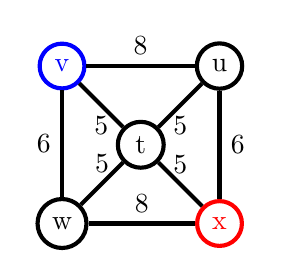
\begin{tikzpicture}[scale = 1, line width = 1.5pt]
\draw (0,2) node[circle,scale = 1, draw, blue](a1){v}
    (2,2) node[circle,scale = 1, draw](a2){u}
    (2,0) node[circle,scale = 1, draw, red](a3){x}
    (0,0) node[circle,scale = 1, draw](a4){w}
    (1,1) node[circle,scale = 1, draw](a5){t};
    \draw [-] (a1) -- (a2) node[midway,scale = 1,above] {8};
    \draw [-] (a1) -- (a4) node[midway,scale = 1,left] {6};
    \draw [-] (a1) -- (a5) node[midway,scale = 1,below] {5};
    \draw [-] (a2) -- (a3) node[midway,scale = 1,right] {6};
    \draw [-] (a2) -- (a5) node[midway,scale = 1,below] {5};
    \draw [-] (a3) -- (a4) node[midway,scale = 1,above] {8};
    \draw [-] (a3) -- (a5) node[midway,scale = 1,above] {5};
    \draw [-] (a4) -- (a5) node[midway,scale = 1,above] {5};
\end{tikzpicture}    
\end{center}

\noindent \begin{table}[]
\centering
\caption{Matriz de Distância de $v-x$}
\label{my-label}
\begin{tabular}{|l|l|l|l|l|l|}
\hline
vértice & peso1                  & peso2 & peso3 & peso4 & peso5\\ \hline
v       & \textcolor{red}{(0,v)} &       &       &  &     \\ \hline
u       &                        &       &       &   &    \\ \hline
w       &                        &       &       &    &   \\ \hline
x       &                        &       &       &     &  \\ \hline
t       &                        &       &       &      & \\ \hline
\end{tabular}
\end{table}
\end{frame}

\begin{frame}{O Algoritmo de Dijkstra}

\begin{center}
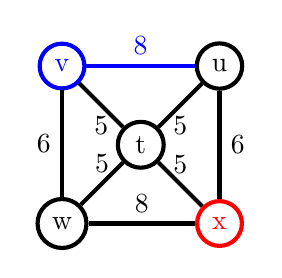
\begin{tikzpicture}[scale = 1, line width = 1.5pt]
\draw (0,2) node[circle,scale = 1, draw, blue](a1){v}
    (2,2) node[circle,scale = 1, draw](a2){u}
    (2,0) node[circle,scale = 1, draw, red](a3){x}
    (0,0) node[circle,scale = 1, draw](a4){w}
    (1,1) node[circle,scale = 1, draw](a5){t};
    \draw [-] (a1) -- (a2)[blue] node[midway,scale = 1,above] {8};
    \draw [-] (a1) -- (a4) node[midway,scale = 1,left] {6};
    \draw [-] (a1) -- (a5) node[midway,scale = 1,below] {5};
    \draw [-] (a2) -- (a3) node[midway,scale = 1,right] {6};
    \draw [-] (a2) -- (a5) node[midway,scale = 1,below] {5};
    \draw [-] (a3) -- (a4) node[midway,scale = 1,above] {8};
    \draw [-] (a3) -- (a5) node[midway,scale = 1,above] {5};
    \draw [-] (a4) -- (a5) node[midway,scale = 1,above] {5};
\end{tikzpicture}    
\end{center}

\noindent \begin{table}[]
\centering
\caption{Matriz de Distância de $v-x$}
\label{my-label}
\begin{tabular}{|l|l|l|l|l|l|}
\hline
vértice & peso1                   & peso2 & peso3 & peso4 & peso5\\ \hline
v       & \textcolor{red}{(0,v)}  &       &       & &      \\ \hline
u       & \textcolor{blue}{(8,v)} &       &       &  &     \\ \hline
w       &                         &       &       &   &    \\ \hline
x       &                         &       &       &    &   \\ \hline
t       &                         &       &       &     &  \\ \hline
\end{tabular}
\end{table}
\end{frame}

\begin{frame}{O Algoritmo de Dijkstra}

\begin{center}
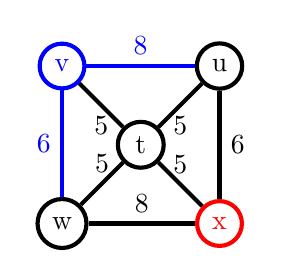
\begin{tikzpicture}[scale = 1, line width = 1.5pt]
\draw (0,2) node[circle,scale = 1, draw, blue](a1){v}
    (2,2) node[circle,scale = 1, draw](a2){u}
    (2,0) node[circle,scale = 1, draw, red](a3){x}
    (0,0) node[circle,scale = 1, draw](a4){w}
    (1,1) node[circle,scale = 1, draw](a5){t};
    \draw [-] (a1) -- (a2)[blue] node[midway,scale = 1,above] {8};
    \draw [-] (a1) -- (a4)[blue] node[midway,scale = 1,left] {6};
    \draw [-] (a1) -- (a5) node[midway,scale = 1,below] {5};
    \draw [-] (a2) -- (a3) node[midway,scale = 1,right] {6};
    \draw [-] (a2) -- (a5) node[midway,scale = 1,below] {5};
    \draw [-] (a3) -- (a4) node[midway,scale = 1,above] {8};
    \draw [-] (a3) -- (a5) node[midway,scale = 1,above] {5};
    \draw [-] (a4) -- (a5) node[midway,scale = 1,above] {5};
\end{tikzpicture}    
\end{center}

\noindent \begin{table}[]
\centering
\caption{Matriz de Distância de $v-x$}
\label{my-label}
\begin{tabular}{|l|l|l|l|l|l|}
\hline
vértice & peso1                   & peso2 & peso3 & peso4 & peso5 \\ \hline
v       & \textcolor{red}{(0,v)}  &       &       & &      \\ \hline
u       & \textcolor{blue}{(8,v)} &       &       &  &     \\ \hline
w       & \textcolor{blue}{(6,v)} &       &       &   &    \\ \hline
x       &                         &       &       &    &   \\ \hline
t       &                         &       &       &     &  \\ \hline
\end{tabular}
\end{table}
\end{frame}

\begin{frame}{O Algoritmo de Dijkstra}

\begin{center}
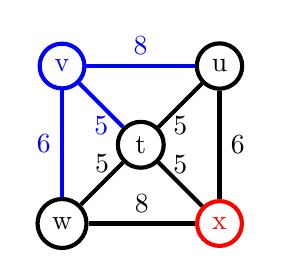
\begin{tikzpicture}[scale = 1, line width = 1.5pt]
\draw (0,2) node[circle,scale = 1, draw, blue](a1){v}
    (2,2) node[circle,scale = 1, draw](a2){u}
    (2,0) node[circle,scale = 1, draw, red](a3){x}
    (0,0) node[circle,scale = 1, draw](a4){w}
    (1,1) node[circle,scale = 1, draw](a5){t};
    \draw [-] (a1) -- (a2)[blue] node[midway,scale = 1,above] {8};
    \draw [-] (a1) -- (a4)[blue] node[midway,scale = 1,left] {6};
    \draw [-] (a1) -- (a5)[blue] node[midway,scale = 1,below] {5};
    \draw [-] (a2) -- (a3) node[midway,scale = 1,right] {6};
    \draw [-] (a2) -- (a5) node[midway,scale = 1,below] {5};
    \draw [-] (a3) -- (a4) node[midway,scale = 1,above] {8};
    \draw [-] (a3) -- (a5) node[midway,scale = 1,above] {5};
    \draw [-] (a4) -- (a5) node[midway,scale = 1,above] {5};
\end{tikzpicture}    
\end{center}

\noindent \begin{table}[]
\centering
\caption{Matriz de Distância de $v-x$}
\label{my-label}
\begin{tabular}{|l|l|l|l|l|l|}
\hline
vértice & peso1                   & peso2 & peso3 & peso4 & peso5 \\ \hline
v       & \textcolor{red}{(0,v)}  &       &       & &      \\ \hline
u       & \textcolor{blue}{(8,v)} &       &       &  &     \\ \hline
w       & \textcolor{blue}{(6,v)} &       &       &   &    \\ \hline
x       &                         &       &       &    &   \\ \hline
t       &\textcolor{blue}{(5,v)}  &       &       &     &  \\ \hline
\end{tabular}
\end{table}
\end{frame}

\begin{frame}{O Algoritmo de Dijkstra}

\begin{center}
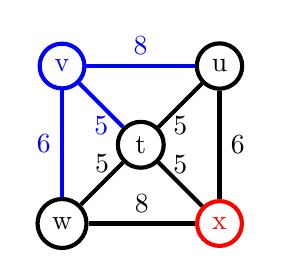
\begin{tikzpicture}[scale = 1, line width = 1.5pt]
\draw (0,2) node[circle,scale = 1, draw, blue](a1){v}
    (2,2) node[circle,scale = 1, draw](a2){u}
    (2,0) node[circle,scale = 1, draw, red](a3){x}
    (0,0) node[circle,scale = 1, draw](a4){w}
    (1,1) node[circle,scale = 1, draw](a5){t};
    \draw [-] (a1) -- (a2)[blue] node[midway,scale = 1,above] {8};
    \draw [-] (a1) -- (a4)[blue] node[midway,scale = 1,left] {6};
    \draw [-] (a1) -- (a5)[blue] node[midway,scale = 1,below] {5};
    \draw [-] (a2) -- (a3) node[midway,scale = 1,right] {6};
    \draw [-] (a2) -- (a5) node[midway,scale = 1,below] {5};
    \draw [-] (a3) -- (a4) node[midway,scale = 1,above] {8};
    \draw [-] (a3) -- (a5) node[midway,scale = 1,above] {5};
    \draw [-] (a4) -- (a5) node[midway,scale = 1,above] {5};
\end{tikzpicture}    
\end{center}

\noindent \begin{table}[]
\centering
\caption{Matriz de Distância de $v-x$}
\label{my-label}
\begin{tabular}{|l|l|l|l|l|l|}
\hline
vértice & peso1                   & peso2                       & peso3 & peso4 & peso5 \\ \hline
v       & \textcolor{red}{(0,v)}  &                             &       &  &     \\ \hline
u       & \textcolor{blue}{(8,v)} &                             &       &   &    \\ \hline
w       & \textcolor{blue}{(6,v)} &                             &       &    &   \\ \hline
x       &                         &                             &       &     &  \\ \hline
t       &\textcolor{blue}{(5,v)}  &  \textcolor{red}{(5,v)}     &       &      & \\ \hline
\end{tabular}
\end{table}
\end{frame}

\begin{frame}{O Algoritmo de Dijkstra}

\begin{center}
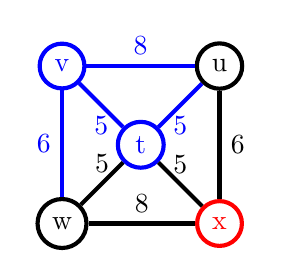
\begin{tikzpicture}[scale = 1, line width = 1.5pt]
\draw (0,2) node[circle,scale = 1, draw, blue](a1){v}
    (2,2) node[circle,scale = 1, draw](a2){u}
    (2,0) node[circle,scale = 1, draw, red](a3){x}
    (0,0) node[circle,scale = 1, draw](a4){w}
    (1,1) node[circle,scale = 1, draw, blue](a5){t};
    \draw [-] (a1) -- (a2)[blue] node[midway,scale = 1,above] {8};
    \draw [-] (a1) -- (a4)[blue] node[midway,scale = 1,left] {6};
    \draw [-] (a1) -- (a5)[blue] node[midway,scale = 1,below] {5};
    \draw [-] (a2) -- (a3) node[midway,scale = 1,right] {6};
    \draw [-] (a2) -- (a5)[blue] node[midway,scale = 1,below] {5};
    \draw [-] (a3) -- (a4) node[midway,scale = 1,above] {8};
    \draw [-] (a3) -- (a5) node[midway,scale = 1,above] {5};
    \draw [-] (a4) -- (a5) node[midway,scale = 1,above] {5};
\end{tikzpicture}    
\end{center}

\noindent \begin{table}[]
\centering
\caption{Matriz de Distância de $v-x$}
\label{my-label}
\begin{tabular}{|l|l|l|l|l|l|}
\hline
vértice & peso1                   & peso2                       & peso3 & peso4 & peso5\\ \hline
v       & \textcolor{red}{(0,v)}  &                             &       &  &     \\ \hline
u       & \textcolor{blue}{(8,v)} & \textcolor{blue}{(10,v)}    &       &   &    \\ \hline
w       & \textcolor{blue}{(6,v)} &                             &       &    &   \\ \hline
x       &                         &                             &       &     &  \\ \hline
t       &\textcolor{blue}{(5,v)}  &  \textcolor{red}{(5,v)}     &       &      & \\ \hline
\end{tabular}
\end{table}
\end{frame}

\begin{frame}{O Algoritmo de Dijkstra}

\begin{center}
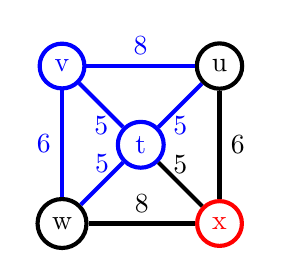
\begin{tikzpicture}[scale = 1, line width = 1.5pt]
\draw (0,2) node[circle,scale = 1, draw, blue](a1){v}
    (2,2) node[circle,scale = 1, draw](a2){u}
    (2,0) node[circle,scale = 1, draw, red](a3){x}
    (0,0) node[circle,scale = 1, draw](a4){w}
    (1,1) node[circle,scale = 1, draw, blue](a5){t};
    \draw [-] (a1) -- (a2)[blue] node[midway,scale = 1,above] {8};
    \draw [-] (a1) -- (a4)[blue] node[midway,scale = 1,left] {6};
    \draw [-] (a1) -- (a5)[blue] node[midway,scale = 1,below] {5};
    \draw [-] (a2) -- (a3) node[midway,scale = 1,right] {6};
    \draw [-] (a2) -- (a5)[blue] node[midway,scale = 1,below] {5};
    \draw [-] (a3) -- (a4) node[midway,scale = 1,above] {8};
    \draw [-] (a3) -- (a5) node[midway,scale = 1,above] {5};
    \draw [-] (a4) -- (a5)[blue] node[midway,scale = 1,above] {5};
\end{tikzpicture}    
\end{center}

\noindent \begin{table}[]
\centering
\caption{Matriz de Distância de $v-x$}
\label{my-label}
\begin{tabular}{|l|l|l|l|l|l|}
\hline
vértice & peso1                   & peso2                       & peso3 & peso4 & peso5\\ \hline
v       & \textcolor{red}{(0,v)}  &                             &       &  &     \\ \hline
u       & \textcolor{blue}{(8,v)} & \textcolor{blue}{(10,v)}    &       &   &    \\ \hline
w       & \textcolor{blue}{(6,v)} & \textcolor{blue}{(10,v)}    &       &    &   \\ \hline
x       &                         &                             &       &     &  \\ \hline
t       &\textcolor{blue}{(5,v)}  &  \textcolor{red}{(5,v)}     &       &      & \\ \hline
\end{tabular}
\end{table}
\end{frame}

\begin{frame}{O Algoritmo de Dijkstra}

\begin{center}
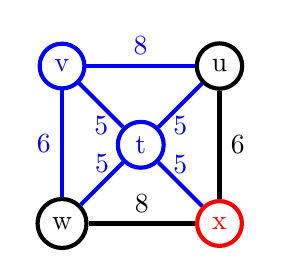
\begin{tikzpicture}[scale = 1, line width = 1.5pt]
\draw (0,2) node[circle,scale = 1, draw, blue](a1){v}
    (2,2) node[circle,scale = 1, draw](a2){u}
    (2,0) node[circle,scale = 1, draw, red](a3){x}
    (0,0) node[circle,scale = 1, draw](a4){w}
    (1,1) node[circle,scale = 1, draw, blue](a5){t};
    \draw [-] (a1) -- (a2)[blue] node[midway,scale = 1,above] {8};
    \draw [-] (a1) -- (a4)[blue] node[midway,scale = 1,left] {6};
    \draw [-] (a1) -- (a5)[blue] node[midway,scale = 1,below] {5};
    \draw [-] (a2) -- (a3) node[midway,scale = 1,right] {6};
    \draw [-] (a2) -- (a5)[blue] node[midway,scale = 1,below] {5};
    \draw [-] (a3) -- (a4) node[midway,scale = 1,above] {8};
    \draw [-] (a3) -- (a5)[blue] node[midway,scale = 1,above] {5};
    \draw [-] (a4) -- (a5)[blue] node[midway,scale = 1,above] {5};
\end{tikzpicture}    
\end{center}

\noindent \begin{table}[]
\centering
\caption{Matriz de Distância de $v-x$}
\label{my-label}
\begin{tabular}{|l|l|l|l|l|l|}
\hline
vértice & peso1                   & peso2                       & peso3 & peso4 & peso5\\ \hline
v       & \textcolor{red}{(0,v)}  &                             &       &  &     \\ \hline
u       & \textcolor{blue}{(8,v)} & \textcolor{blue}{(10,v)}    &       &   &    \\ \hline
w       & \textcolor{blue}{(6,v)} & \textcolor{blue}{(10,v)}    &       &    &   \\ \hline
x       &                         & \textcolor{blue}{(10,v)}    &       &     &  \\ \hline
t       &\textcolor{blue}{(5,v)}  &  \textcolor{red}{(5,v)}     &       &      & \\ \hline
\end{tabular}
\end{table}
\end{frame}

\begin{frame}{O Algoritmo de Dijkstra}

\begin{center}
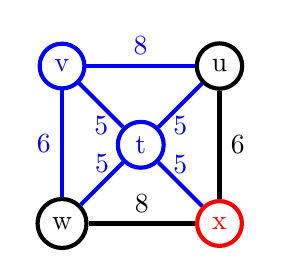
\begin{tikzpicture}[scale = 1, line width = 1.5pt]
\draw (0,2) node[circle,scale = 1, draw, blue](a1){v}
    (2,2) node[circle,scale = 1, draw](a2){u}
    (2,0) node[circle,scale = 1, draw, red](a3){x}
    (0,0) node[circle,scale = 1, draw](a4){w}
    (1,1) node[circle,scale = 1, draw, blue](a5){t};
    \draw [-] (a1) -- (a2)[blue] node[midway,scale = 1,above] {8};
    \draw [-] (a1) -- (a4)[blue] node[midway,scale = 1,left] {6};
    \draw [-] (a1) -- (a5)[blue] node[midway,scale = 1,below] {5};
    \draw [-] (a2) -- (a3) node[midway,scale = 1,right] {6};
    \draw [-] (a2) -- (a5)[blue] node[midway,scale = 1,below] {5};
    \draw [-] (a3) -- (a4) node[midway,scale = 1,above] {8};
    \draw [-] (a3) -- (a5)[blue] node[midway,scale = 1,above] {5};
    \draw [-] (a4) -- (a5)[blue] node[midway,scale = 1,above] {5};
\end{tikzpicture}    
\end{center}

\noindent \begin{table}[]
\centering
\caption{Matriz de Distância de $v-x$}
\label{my-label}
\begin{tabular}{|l|l|l|l|l|l|}
\hline
vértice & peso1                   & peso2                       & peso3                    & peso4 & peso5\\ \hline
v       & \textcolor{red}{(0,v)}  &                             &                          &  &     \\ \hline
u       & \textcolor{blue}{(8,v)} & \textcolor{blue}{(10,v)}    &                          &   &    \\ \hline
w       & \textcolor{blue}{(6,v)} & \textcolor{blue}{(10,v)}    &                          &    &   \\ \hline
x       &                         & \textcolor{blue}{(10,v)}    & \textcolor{red}{(10,v)}  &     &  \\ \hline
t       &\textcolor{blue}{(5,v)}  &  \textcolor{red}{(5,v)}     &                          &      & \\ \hline
\end{tabular}
\end{table}
\end{frame}

\begin{frame}{O Algoritmo de Dijkstra}
    \begin{alertblock}{Achamos o Caminho!!}
        A partir daí, é obvio perceber que qualquer outro caminho que tomemos terá uma distância maior que dez, visto que, já que chegamos ao nosso destino (único), qualquer outro caminho que tomássemos teria que ter uma aresta de peso maior que zero!! Resta, agora, repetirmos o procedimento para construirmos uma matriz D para todos os vértices ímpares $v_{i}-v_{j}$. 
    \end{alertblock}
    
\end{frame}

\begin{frame}{A Matriz de Distância}
\section{A Matriz de Distância}
    \begin{center}
        \begin{table}[]
\centering
\caption{A Matriz de Distância}
\label{my-label}

\scalebox{0.7}{
\begin{tabular}{|l|l|l|l|l|}
\hline
\cellcolor[HTML]{EFEFEF} & v                         & u                         & w                         & x                         \\ \hline
v                        & \cellcolor[HTML]{EFEFEF}0 & 8                         & 6                         & 10                        \\ \hline
u                        & 8                         & \cellcolor[HTML]{EFEFEF}0 & 10                        & 6                         \\ \hline
w                        & 6                         & 10                        & \cellcolor[HTML]{EFEFEF}0 & 8                         \\ \hline
x                        & 10                        & 6                         & 8                         & \cellcolor[HTML]{EFEFEF}0 \\ \hline
\end{tabular}}
\end{table}
    \end{center}
    \begin{enumerate}[3]
        \item A partir da matriz D, fazemos uma analise combinatória simples entre as distancias dos vértices ímpares, para determinarmos o menor caminho entre eles e adicionarmos as arestas ``artificiais'':
    \end{enumerate}
    \begin{itemize}
        \item v-u + w-x = 8 + 8 = 16
        \item v-x + u-w = 10 + 10 = 20
        \item v-w + u-x = 6 + 6 = 12
    \end{itemize}
    
\end{frame}

\begin{frame}{Criando as Arestas Artificiais}
\begin{enumerate}[4]
    \item Criamos, então, as arestas artificiais com seus respectivos pesos, já acrescidos: 
\end{enumerate}

\begin{center}
    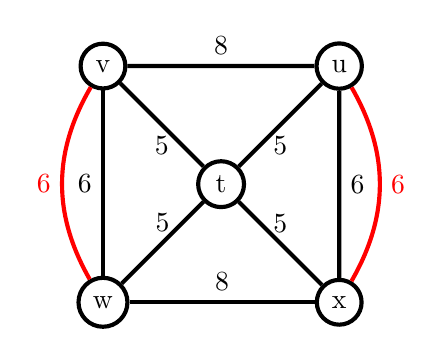
\begin{tikzpicture}[scale = 1.5, line width = 1.5pt]
\draw (0,2) node[circle, draw](a1){v}
    (2,2) node[circle, draw](a2){u}
    (2,0) node[circle, draw](a3){x}
    (0,0) node[circle, draw](a4){w}
    (1,1) node[circle, draw](a5){t};
    
    \path[-] (a1) edge node[above] {8} (a2);
    \path[-] (a1) edge node[left] {6} (a4);
    \path[-] (a1) edge [bend right = 30, red] node[left, red] {6} (a4);
    \path[-] (a1) edge node[below] {5} (a5);
    \path[-] (a2) edge node[below] {5} (a5);
    \path[-] (a3) edge node[above] {5} (a5);
    \path[-] (a4) edge node[above] {5} (a5);
    \path[-] (a4) edge node[above] {8} (a3);
    \path[-] (a2) edge node[right] {6} (a3);
    \path[-] (a2) edge [bend left = 30, red] node[right, red] {6} (a3);
    
\end{tikzpicture}    
\end{center}

De tal forma que o grafo agora se torna euleriano, tendo, então, uma solução optimal.   
    
\end{frame}

\begin{frame}{A Solução}
\section{A Solução}

\begin{enumerate}[5]
    \item Eliminar da matriz D as colunas e linhas correspondentes a $v_{i}$ e $v_{j}$.
\end{enumerate}
\begin{enumerate}[6]
    \item Se ainda assim houver vértices ímpares, retornar ao passo 3.
\end{enumerate}
\begin{enumerate}[7]
    \item O custo total percorrido será igual ao custo inicial do grafo G somado com o custo das arestas acrescidas.
\end{enumerate}

A partir do momento que tornamos o grafo não euleriano num grafo euleriano, a solução do problema se torna o custo da soma de todas as arestas originais do grafo acrescida do custo das arestas ``artificiais'' criadas. Assim, o custo total desse grafo é 60.
    
\end{frame}

\begin{frame}{Aplicações Práticas}
\section{Aplicações Práticas}

Várias são as aplicações do problema do carteiro chinês - como já dito anteriormente. Podemos, aqui, exemplificar algumas delas:
    \begin{itemize}
        \item Dado um bairro B, um entregador de jornais entrega de bicicleta jornais pelas casas da vizinhança. Sendo as ruas as arestas e as casas os vértices, como esse entregador pode maximizar seu tempo de entrega, levando em consideração o ``comprimento'' das ruas como os pesos?
        \item Dado uma cidade C, uma empresa de coleta de lixo precisa passar por determinados pontos P de coleta, passando por determinadas ruas. Cada rua tem um comprimento diferente e são \textbf{direcionadas}. Como essa empresa montará uma rota de coleta minimizando os custos? 
   \end{itemize}

\end{frame}

\begin{frame}{Conclusão}
\section{Conclusao}
    Considerando todos esses exemplos grafos conexos e não-Eulerianos, embora somente o primeiro tenha solução da forma como apresentada aqui, o outros é, também, variante do problema do carteiro chinês. Um paper de mestrado da Universidade de Amsterdam do estudante Jozefien Karskens, orientado pelo professor Dr. R. Bekker apresenta o mesmo problema (um exemplo real) e suas variantes, e o soluciona.\footnote{https://beta.vu.nl/nl/Images/researchpaper-karskens\_tcm235-363659.pdf}
    
\end{frame}

\begin{frame}{Conclusão}
Aqui foi mostrado o algoritmo da solução do problema do carteiro chinês para um grafo não direcionado e com pesos \textit{\textbf{positivos}} nas arestas. Esse problema possui outras várias variantes e as aplicações no ``\textit{mundo real}'' são extremamentes distintas, como já dito anteriormente.\\
    As referências bibliográficas desse trabalho foram majoritariamente oriundas de videos e artigos. O pacote utilizado para a confecção dos grafos foi o \textit{TIKZ}.
\end{frame}

\end{document}

